% Hopefully this will be the final version of Problem statement.
This chapter introduces this research proposal. It starts with the problem statement, then outlines the motivations, research goals and the organization of this proposal.

\section{Problem Statement}
\label{sec:statement}
% \bx{what is cloud computing and why it is the pillar of software and other related industry. (importance of cloud computing.)}
% \bx{
% \begin{itemize}
% 	\item (what) the main challenge for cloud provider is to reduce energy consumption
% 	\item why it is important and so what? (consequences?),
% 	\item how to deal with it? (technologies)
% \end{itemize}}
\bx{Cloud computing has made a huge impact on modern software industry by offering on-demand computing capacity 
(e.g storage and computing) \cite{2010arxiv1006.0308b}.} Compared with the traditional software industry, where applications run
on individual hardware, on-demand cloud computing provides convenient architectures for the software industry. For example, 
web service providers such as Google and Neflix deploy their applications on cloud. These web service providers 
do not need to purchase and maintain hardware resources. 
In addition, they do not need to worry 
about scalability and availability issues when demands of their applications increase. Cloud dynamically increases the capacity of applications and cloud computing services are accessible 99.99\% of the time ~\cite{adhikari:2012uq}.
% \sout{can develop, deploy and maintain applications (e.g. google drive) on cloud  without worrying about.} 
\qy{Moreover, application users} can enjoy applications without experiencing breakdown and access the applications from anywhere in the world.

\bx{A major issue in cloud computing is the huge energy consumption generated by data centers.}
A typical data center consumes as much energy as 25,000 households \cite{dayarathna:2016ua}. 
This huge energy consumption has become the major expense of cloud providers. It is necessary to find ways to reduce the energy bills. 
The reduction of energy bills would benefit to both \qy{cloud providers and web service providers.} 
% \sout{to the profit in software industry.} 
Furthermore, people would pay less to applications on the \qy{cloud}. 

\bx{Generally, reducing the energy consumption in cloud depends on
improving the resource utilization of live physical machines (PMs) such as servers.} 
Studies show \cite{Barroso:2007jt, Shen:2015hm}, \qy{PMs account for} \qy{the majority} -- more than 40\% -- of energy consumption \qy{in cloud among other components such as cooling systems and network devices}. \qy{Moreover},
these PMs has been not used effectively. \qy{Some studies analyzed that }the proportion of PMs' average utilization is quite low 
- from 10\% to 50\% \cite{Hameed:2016cmb} 
% \sout{due to some disadvantages in resource management}. 
Therefore, we need to reduce energy by improving the utilization of PMs \qy{and reducing the usage of PMs in cloud}.
% This is because cloud users tend to preserve more resources in order to guarantee the performance when facing the variation of workloads.

\bx{The common way to improve the utilization of PMs in cloud 
is through resource management of PMs \cite{Manvi:2014hm} (see Figure \ref{fig:workflow}).} 
% \sout{The cloud resource management of PMs is a centralized system \cite{Jennings:2015ht}. The management system} 
\qy{ A centralized resource management system in cloud}
has two \qy{main} functionalities. \qy{First, the management} system 
allocates resources such as CPUs and memories of PMs \qy{for} cloud users \qy{to run} applications. \qy{Second, the management} system 
handles the workload fluctuations \qy{to reduce the potential migration}. \qy{These two main functionalities deploy and maintain applications in cloud.} 

\bx{The two main functionalities of resource management of PMs in cloud involve four steps.}
First, the management system collects the utilization information of PMs and then 
analyze the usage of PMs and the resource needed by applications. Next, triggered by resource analysis, the management system determines the 
placement of applications. The placement of applications includes three scenarios: initial placement of application for new applications; periodic placement of application for adjusting the placement periodically; 
and dynamic placement of application for adjusting applications in a fast manner when abnormal events such as overloading happen. Finally, 
the management system executes the placement decision of applications to PMs. Hence, better management of resources 
in cloud contributes towards a better utilization of PMs and thus a reduction of energy consumption.


% \sout{Four major steps in resource management are listed as follows: Collecting utilization data from PMs, analyzing 
% available resources on PMs, deciding the placement of applications on PMs, and executing the application placement decisions.  
% As better allocation of CPUs and memories leads to a reduction of energy consumption, the placement decision is the most important step.}

% \sout{\bx{Placement decision is applied in three scenarios to improve the utilization of PMs.} Three placement 
% decision scenarios are common in a data center: initial placement of application handles new arrival of applications; periodic placement of 
% application adjusts the placement globally and periodically; dynamic placement of application adjusts application in a fast manner. 
% All three decision scenarios rely on an optimization strategy called server consolidation.}  



\begin{figure}
	\centering
	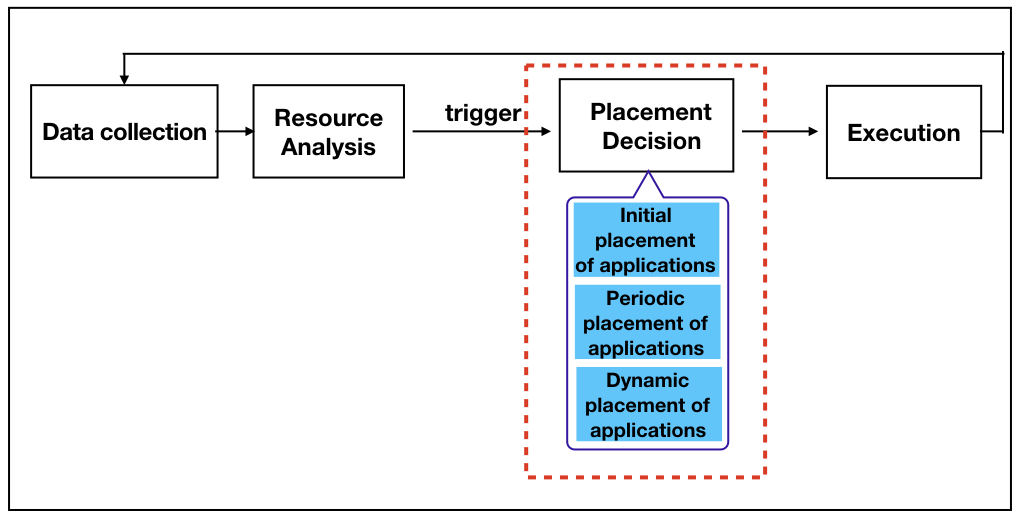
\includegraphics[width=0.8\textwidth]{pics/workflow_management.png}
	\caption{A workflow of resource management \cite{Mishra:2012kx}}
	\label{fig:workflow}
\end{figure}

% Data collection gathers resource utilization information from individual PMs and VMs such as CPU, memory utilization in a period of time. These data are collected by monitoring softwares for data analysis. Data analysis takes the collected data as the input, cleans and analyzes them. It outputs the quantity of demand resources of applications. Finally, execution places the applications to the target PMs. 

% \bx{Among these resource management steps, placement decision is the crucial step which includes three scenarios: initial placement of application, periodic placement of application and overloading & under-loading adjustment.} Essentially, these three scenarios contain a common strategy called server consolidation.


% \sout{Server consolidation \cite{Varasteh:2015fu} is a \qy{popular} strategy to manage the resources of PMs 
% by placing applications in fewer PMs and lead to lower energy consumption.
% For three resource management scenarios, they are generally considered as two types of problem: 
% static and dynamic. Static problem is solved in an off-line fashion which includes initial placement of 
% application and periodic placement of application. Dynamic placement of application problem is solved in an on-line fashion. 
% In order to solve static and dynamic problems, server consolidation strategy must also be designed in static and dynamic fashions.}

\bx{The core strategy of resource management is server consolidation \cite{Varasteh:2015fu}.} Two different types of
server consolidation are used in cloud: static and dynamic. Static server consolidation manages resources in an off-line fashion. It is mainly 
used in the initial placement of applications and periodic placement of applications. Dynamic server consolidation manages resources in 
an on-line fashion, which is used in the dynamic placement of applications. Both static and dynamic server consolidation aim to place
applications in fewer PMs. This leads to higher utilization of PMs and lower energy consumption.


% \sout{\bx{Currently, resource management in data centers is based on \emph{virtualization} technology\cite{Uhlig:2005do}.} 
% Such virtualization separates the resources (e.g. CPUs and RAMs) of a PM into several parts called \emph{virtual machines (VMs)}, 
% each of VMs runs an isolated operating system. Compare with virtualization, the traditional data center places an application to 
% a single PM. The traditional placement leads to the low utilization of PMs. After the technique of VM being introduced, 
% the multiplexing of PMs largely improves the utilization and reduces the energy consumption.} 

\bx{Currently, the resource management in cloud is based on \emph{virtualization} technology\cite{Uhlig:2005do} and the mainstream is virtual machine-based virtualization.}
Such virtualization separates the resources (e.g. CPUs and RAMs) of a PM into several parts called \emph{virtual machines (VMs)}. 
Each VM runs an isolated operating system. This VM-based technology is very different from a 
traditional cloud that places each application to a single PM and leads to the low reserved utilization of PMs. 
Compared with traditional clouds, current VM-based clouds significantly improve the utilization of PMs and reduce energy consumption.

% \sout{However, in recent years, resource management with VMs cannot catch up with a new trend in 
% software industry -- Service Oriented Architecture 
% (SOA) \cite{Sprott:2004wt}; SOA has become widely used in modern software industry because of its agility and re-usability \cite{Sprott:2004wt}.
% SOA separates a centralized application into multiple distributed components called web services. 
% As most of web services only require a small amount of resources (e.g. 15\% of CPU), 
% using a VM for a web service causes resource wastage inside a VM. Consequently, the low utilization of PMs decreases
% the energy efficiency. To support the architecture of SOA and further reduce energy consumption, a new virtualization 
% technology: containers \cite{Felter:2015ki, Soltesz:2007cu} has been proposed. The container technology provides a new 
% architecture for allocating applications and a finer granularity of resource management. Containers has the potential to further
% improve the energy consumption.}


\bx{However, in recent years, virtual machine-based virtualization cannot catch up with a new trend in the software industry -- Service Oriented Architecture 
(SOA) \cite{Sprott:2004wt}.} This SOA is widely used in modern software industry because of its agility and re-usability \cite{Sprott:2004wt}.
SOA separates a centralized application into multiple distributed components called web services. 
As web services only require a small amount of resources (e.g. 15\% of CPU), 
using a VM for a web service causes resource wastage inside a VM. Consequently, the low utilization of PMs decreases
the energy efficiency.


\bx{To support the architecture of SOA and further reduce energy consumption, a new container-based virtualization \cite{Felter:2015ki, Soltesz:2007cu} has been proposed.} Containers running on top of 
VMs are called an operating system (OS) level of virtualization \cite{Soltesz:2007cu}. Similar to VM, 
a container provides performance and resource isolation for a single application. 
Different to VMs, multiple containers can run in the same VM without interfering with each other. 
In addition, containers naturally support vertical scaling (change size during runtime)\cite{Vaquero:2011gb}. 
The vertical scaling provides resilient resources to fluctuate workloads. The container technology provides a new 
architecture for allocating applications and a finer granularity of resource management. Hence, containers have the potential to further
improve the energy consumption.



\bx{Although the efficient use of containers can improve the utilization of VMs, 
containers bring new challenges and difficulties to server consolidation \cite{:2017ff}. }
We cannot directly apply current VM-based server consolidation strategies on container-based clouds because 
of the different placement structures of applications. Moreover, to support the increasing size of containers, 
the vertical scaling in cloud requires the VMs to reserve sufficient resources. The interaction between VMs and containers changes 
the server consolidation into a bilevel problem: VMs-to-PMs, and VMs-to-containers. Bilevel problems are NP-hard~\cite{Sinha:2013tn}.  NP-hard means it is difficult for a polynomial algorithm to find the global optimum solution. Therefore, we need to develop better algorithms for the bilevel problem.

\bx{This research aims at improving the energy efficiency in container-based clouds by 
proposing new bilevel energy models and server consolidation algorithms for three placement decision scenarios: }
initial placement of application, periodic placement of application, and dynamic placement of application.




% In summary, in order to improve energy efficiency in container-based data center, this research aims at proposing new models and algorithms for three placement decision scenarios:initial placement of application, periodic placement of application, and dynamic placement of application. In the following section, we will discuss the challenges in these scenarios.

% \bx{Despite which virtualization is used, server consolidation can be applied in three resource management scenarios:} initial placement of application  \cite{Jennings:2015ht}, periodic placement of application \cite{Mishra:2012kx} and overloading/under-loading adjustments \cite{Mishra:2012kx} (see Figure \ref{fig:workflow}).

 % Server consumption is essentially an optimization task where it adjusts applications' locations in PMs so that a minimum number of PMs is used. For a certain number of applications, the fewer number of PMs is used, the less energy is consumed. 

% Three management processes: initial placement of application, periodic placement of application ,   have distinct characteristics, hence, the server consolidation techniques applied on them can be roughly classified into two categories: static \cite{Xiao:2015ik} and dynamic \cite{Beloglazov:2012bw}.

% \bx{In Initial application placement, the consolidation can be described as a static task conducted in an off-line manner.} 
\vspace{5mm}
